\documentclass[tikz,border=5pt]{standalone}
\usepackage[T1]{fontenc}
\usepackage{lmodern,amsmath,amssymb}
\usetikzlibrary{arrows.meta,calc,positioning,fit,backgrounds,shapes.geometric,matrix,decorations.pathreplacing,patterns}
\definecolor{ink}{gray}{0.08}
\definecolor{wash}{gray}{0.965}
\definecolor{soft}{gray}{0.45}
\tikzset{box/.style={draw=ink,line width=.65pt,fill=white,align=center,inner sep=4pt,outer sep=0pt,font=\small},flow/.style={draw=ink,line width=.65pt,-{Latex[length=1.8mm,width=1.3mm]},rounded corners=2pt},annotation/.style={font=\scriptsize,text=soft,align=center},groupbox/.style={draw=soft,dashed,line width=.45pt,fill=wash}}
\begin{document}
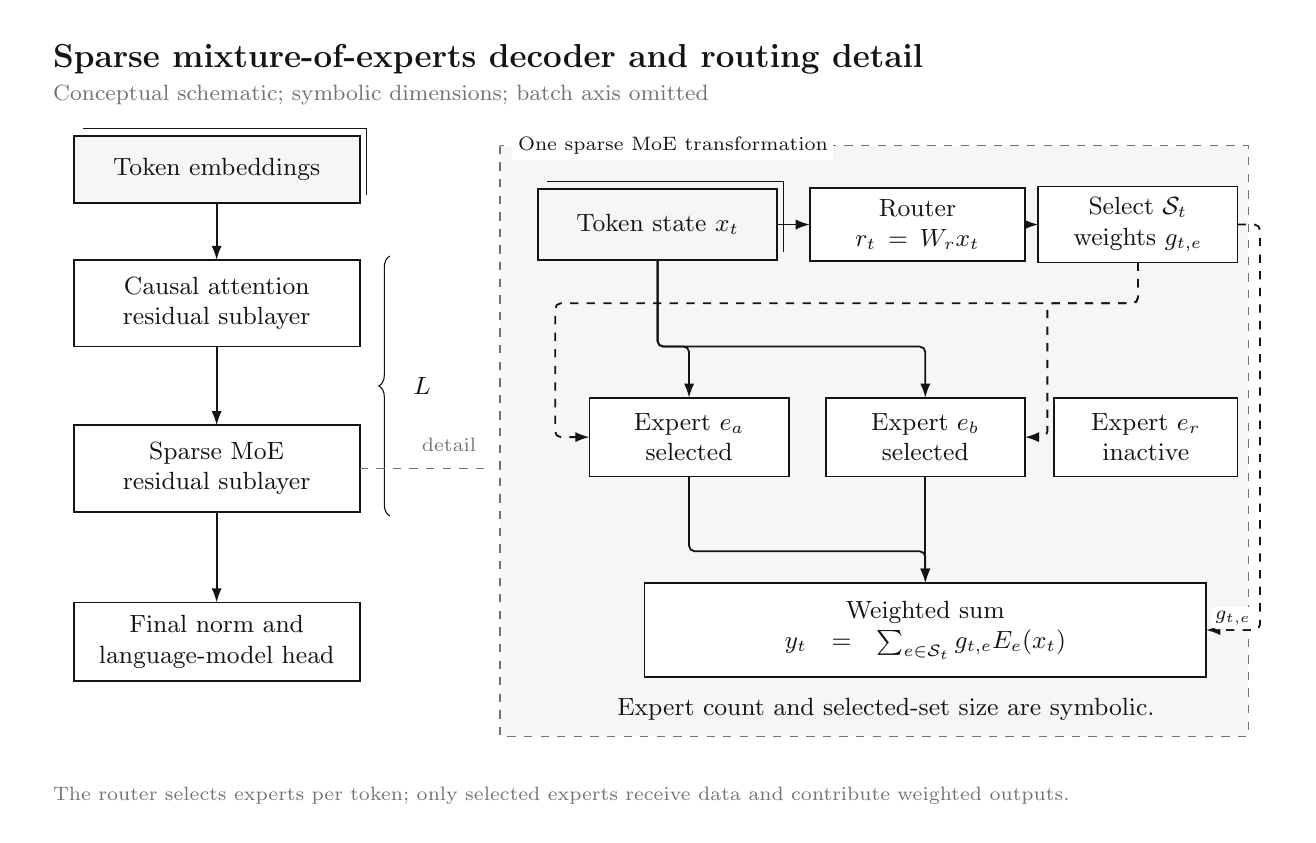
\begin{tikzpicture}[x=1cm,y=-1cm,font=\rmfamily,text=ink]

\path[use as bounding box] (0,0) rectangle (16,10);
\node[anchor=west,font=\large\bfseries] at (.2,.4) {Sparse mixture-of-experts decoder and routing detail};
\node[anchor=west,font=\footnotesize,text=soft] at (.2,.85) {Conceptual schematic; symbolic dimensions; batch axis omitted};
\begin{pgfonlayer}{background}
\draw[groupbox] (6.0,1.5) rectangle (15.5,9.0);
\node[anchor=west,font=\scriptsize,fill=white,inner sep=2pt] at (6.15,1.5) {One sparse MoE transformation};
\end{pgfonlayer}
\node[box,fill=wash,minimum width=3.6cm,minimum height=0.85cm,text width=3.35cm] (tokens) at (2.4,1.8) {Token embeddings};
\draw[ink,line width=.4pt] (0.6999999999999998,1.275) -- (4.3,1.275) -- (4.3,2.125);
\node[box,minimum width=3.6cm,minimum height=1.1cm,text width=3.35cm] (attn) at (2.4,3.5) {Causal attention\\residual sublayer};
\node[box,minimum width=3.6cm,minimum height=1.1cm,text width=3.35cm] (moe) at (2.4,5.6) {Sparse MoE\\residual sublayer};
\node[box,minimum width=3.6cm,minimum height=1.0cm,text width=3.35cm] (head) at (2.4,7.8) {Final norm and\\language-model head};
\node[box,fill=wash,minimum width=3.0cm,minimum height=0.9cm,text width=2.75cm] (x) at (8.0,2.5) {Token state $x_t$};
\draw[ink,line width=.4pt] (6.6,1.9499999999999997) -- (9.6,1.9499999999999997) -- (9.6,2.85);
\node[box,minimum width=2.7cm,minimum height=0.9cm,text width=2.45cm] (router) at (11.3,2.5) {Router\\$r_t=W_rx_t$};
\node[box,minimum width=2.5cm,minimum height=0.9cm,text width=2.25cm] (topk) at (14.1,2.5) {Select $\mathcal S_t$\\weights $g_{t,e}$};
\node[box,minimum width=2.5cm,minimum height=1.0cm,text width=2.25cm] (ea) at (8.4,5.2) {Expert $e_a$\\selected};
\node[box,minimum width=2.5cm,minimum height=1.0cm,text width=2.25cm] (eb) at (11.4,5.2) {Expert $e_b$\\selected};
\node[box,minimum width=2.3cm,minimum height=1.0cm,text width=2.05cm] (er) at (14.2,5.2) {Expert $e_r$\\inactive};
\node[box,minimum width=7.1cm,minimum height=1.2cm,text width=6.85cm] (sum) at (11.4,7.65) {Weighted sum\\$y_t=\sum_{e\in\mathcal S_t}g_{t,e}E_e(x_t)$};
\node[align=center,inner sep=0pt,outer sep=0pt,font=\small,minimum width=8.7cm,minimum height=0.4cm,text width=8.45cm] (note11) at (10.9,8.65) {Expert count and selected-set size are symbolic.};
\begin{pgfonlayer}{background}
\draw[flow] (tokens.south) -- (attn.north);
\draw[flow] (attn.south) -- (moe.north);
\draw[flow] (moe.south) -- (head.north);
\draw[flow] (x.east) -- (router.west);
\draw[flow] (router.east) -- (topk.west);
\draw[flow] (x.south) -- (8,4.05) -- (8.4,4.05) -- (ea.north);
\draw[flow] (x.south) -- (8,4.05) -- (11.4,4.05) -- (eb.north);
\draw[flow,dashed] (topk.south) -- (14.1,3.5) -- (6.7,3.5) -- (6.7,5.2) -- (ea.west);
\draw[flow,dashed] (topk.south) -- (14.1,3.5) -- (12.95,3.5) -- (12.95,5.2) -- (eb.east);
\draw[flow,dashed] (topk.east) -- (15.65,2.5) -- (15.65,7.65) -- (sum.east) node[midway,above,fill=white,inner sep=1.5pt,font=\scriptsize] {$g_{t,e}$};
\draw[flow] (ea.south) -- (8.4,6.65) -- (11.4,6.65) -- (sum.north);
\draw[flow] (eb.south) -- (sum.north);
\end{pgfonlayer}
\draw[decorate,decoration={brace,amplitude=4pt},draw=ink] (4.6,6.2)--(4.6,2.9) node[midway,right=5pt,font=\small] {$L$};
\draw[draw=soft,dashed,line width=.45pt] (moe.east)--(5.85,5.6);\node[annotation] at (5.35,5.3) {detail};
\node[anchor=west,align=left,font=\scriptsize,text=soft,text width=15.6cm] at (.2,9.75) {The router selects experts per token; only selected experts receive data and contribute weighted outputs.};
\end{tikzpicture}
\end{document}
